\documentclass[tikz,border=10pt]{standalone}
\usepackage{tikz}
\usetikzlibrary{decorations.markings, calc}

\begin{document}

% Q1
\begin{tikzpicture}[scale=1, transform shape,
    % Define the style for the mid arrow
    midarrow/.style={
        decoration={markings, mark=at position 0.5 with {\arrow[line width=0.5mm]{>}}},
        postaction={decorate}
    }
]

% Define the points of the triangle
\coordinate (O) at (0,0);
\coordinate (A) at (4,3);
\coordinate (B) at (5,0);

% Draw the triangle with labels
\draw (O) -- (A) node[midway, above left] {$a$};
\draw (O) -- (B) node[midway, below] {$b$};
\draw (A) -- (B);

% Add the points labels
\node at (O) [left] {O};
\node at (A) [above] {A};
\node at (B) [right] {B};

% Draw the mid arrows
\draw[midarrow] (O) -- (A);
\draw[midarrow] (O) -- (B);

\end{tikzpicture}

% Q2
\begin{tikzpicture}[scale=1, transform shape,
    % Define the style for the mid arrow
    midarrow/.style={
        decoration={markings, mark=at position 0.5 with {\arrow[line width=0.5mm]{>}}},
        postaction={decorate}
    }
]

% Define the points of the triangle
\coordinate (O) at (0,0);
\coordinate (A) at (4,3);
\coordinate (B) at (5,0);

% Draw the triangle with labels
\draw (O) -- (A) node[midway, above left] {$3a$};
\draw (O) -- (B) node[midway, below] {$5b$};
\draw (A) -- (B);

% Add the points labels
\node at (O) [left] {O};
\node at (A) [above] {A};
\node at (B) [right] {B};

% Draw the mid arrows
\draw[midarrow] (O) -- (A);
\draw[midarrow] (O) -- (B);

\end{tikzpicture}

% Q3
\begin{tikzpicture}[scale=1, transform shape,
    % Define the style for the mid arrow
    midarrow/.style={
        decoration={markings, mark=at position 0.5 with {\arrow[line width=0.5mm]{>}}},
        postaction={decorate}
    }
]

% Define the points of the triangle
\coordinate (O) at (0,0);
\coordinate (A) at (4,3);
\coordinate (B) at (5,0);

% Draw the triangle with labels
\draw (O) -- (A) node[midway, above left] {$a$};
\draw (O) -- (B) node[midway, below] {$2b$};
\draw (A) -- (B);

% Add the points labels
\node at (O) [left] {O};
\node at (A) [above] {A};
\node at (B) [right] {B};

% Draw the mid arrows
\draw[midarrow] (O) -- (A);
\draw[midarrow] (O) -- (B);

\end{tikzpicture}

% Q4
\begin{tikzpicture}[scale=1, transform shape,
    % Define the style for the mid arrow
    midarrow/.style={
        decoration={markings, mark=at position 0.5 with {\arrow[line width=0.5mm]{>}}},
        postaction={decorate}
    }
]

% Define the points of the triangle
\coordinate (O) at (0,0);
\coordinate (A) at (4,3);
\coordinate (B) at (5,0);
\coordinate (C) at (7,0);

% Draw the triangle with labels
\draw (O) -- (A) node[midway, above left] {$5a$};
\draw (O) -- (B) node[midway, below] {$3b$};
\draw (A) -- (B);
\draw (B) -- (C);

% Add the points labels
\node at (O) [below] {O};
\node at (A) [above] {A};
\node at (B) [below] {B};
\node at (C) [below] {C};

% Draw the mid arrows
\draw[midarrow] (O) -- (A);
\draw[midarrow] (O) -- (B);
\node at (B) [below] {B};

\% Mark the points M (midway between A and B), and C with dots
\fill[black] ($(A)!0.5!(B)$) circle (2pt) node[above right] {D};
\fill[black] (C) circle (2pt);

\end{tikzpicture}


% Q5
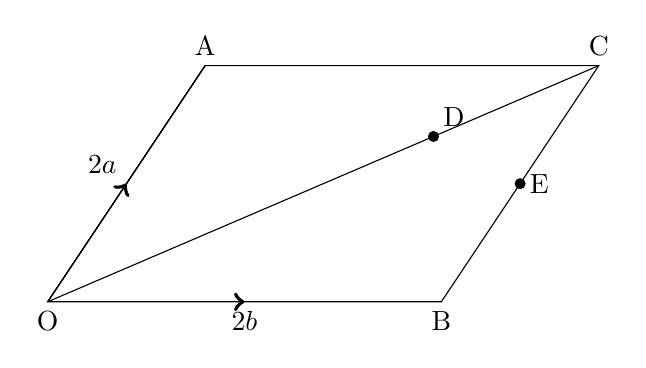
\begin{tikzpicture}[scale=1, transform shape,
    % Define the style for the mid arrow
    midarrow/.style={
        decoration={markings, mark=at position 0.5 with {\arrow[line width=0.5mm]{>}}},
        postaction={decorate}
    }
]

% Define the points of the triangle
\coordinate (O) at (0,0);
\coordinate (A) at (2,3);
\coordinate (B) at (5,0);
\coordinate (C) at (7,3);


% Draw the lines
\draw (O) -- (A) -- (C) -- (B) -- cycle;
\draw (O) -- (A) node[midway, above left] {$2a$};
\draw (O) -- (B) node[midway, below] {$2b$};
\draw (O) -- (C);


% Add the points labels
\node at (O) [below] {O};
\node at (A) [above] {A};
\node at (B) [below] {B};
\node at (C) [above] {C};

% Draw the mid arrows
\draw[midarrow] (O) -- (A);
\draw[midarrow] (O) -- (B);

\% Mark the points D (midway between A and B), and C with dots
\fill[black] ($(O)!0.7!(C)$) circle (2pt) node[above right] {D};
\fill[black] ($(C)!0.5!(B)$) circle (2pt) node[right] {E};

\end{tikzpicture}


% Q6
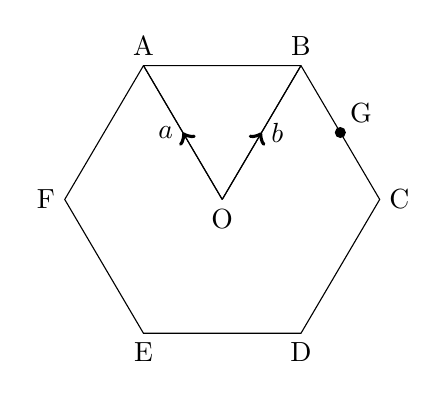
\begin{tikzpicture}[scale=1, transform shape,
    % Define the style for the mid arrow
    midarrow/.style={
        decoration={markings, mark=at position 0.5 with {\arrow[line width=0.5mm]{>}}},
        postaction={decorate}
    }
]

% Define the points of the triangle
\coordinate (O) at (0,0);
\coordinate (A) at (-1,1.7);
\coordinate (B) at (1,1.7);
\coordinate (C) at (2,0);
\coordinate (D) at (1,-1.7);
\coordinate (E) at (-1,-1.7);
\coordinate (F) at (-2,0);


% Draw the lines
\draw (A) -- (B) -- (C) -- (D) -- (E) -- (F) -- cycle;
\draw (O) -- (A) node[midway, left] {$a$};
\draw (O) -- (B) node[midway, right] {$b$};


% Add the points labels
\node at (O) [below] {O};
\node at (A) [above] {A};
\node at (B) [above] {B};
\node at (C) [right] {C};
\node at (D) [below] {D};
\node at (E) [below] {E};
\node at (F) [left] {F};

% Draw the mid arrows
\draw[midarrow] (O) -- (A);
\draw[midarrow] (O) -- (B);

\% Mark the points D (midway between A and B), and C with dots
\fill[black] ($(B)!0.5!(C)$) circle (2pt) node[above right] {G};

\end{tikzpicture}

\end{document}
